\documentclass[t]{beamer}
\usepackage{mathtools}
\usepackage{tikz}
\usepackage{pgfplots}
\usepackage{ulem}
\usetikzlibrary{arrows,backgrounds,shapes,matrix,positioning,fit}
\newcommand{\argmax}{\operatornamewithlimits{argmax}}
\newcommand{\argmin}{\operatornamewithlimits{argmin}}
\newcommand{\wt}{\operatornamewithlimits{wt}}
\renewcommand\Re{\operatorname{Re}}
\renewcommand\Im{\operatorname{Im}}

\mode<presentation>
{
  \usetheme{Singapore}
  %\useoutertheme{infolines} % Showing only current section in navigation
  \setbeamertemplate{headline}{}  % Empty headline
  \setbeamertemplate{footline}[frame number]  % Getting rid of footer items except slide number
  \setbeamercovered{invisible}
  \beamertemplatenavigationsymbolsempty % Getting rid of navigation bullets at the bottom
}
\usepackage[english]{babel}
\usepackage[latin1]{inputenc}
\usepackage{times}
\usepackage[T1]{fontenc}

\title[EE 703 DMT]{Power Spectral Density of Digitally Modulated Signals}
\author[Saravanan V]
{
  Saravanan Vijayakumaran\\
  \href{mailto:sarva@ee.iitb.ac.in}{sarva@ee.iitb.ac.in}
}
\institute[IIT Bombay]
{
  Department of Electrical Engineering\\
  Indian Institute of Technology Bombay
}
\date{August 22, 2013}

\AtBeginSection[]%
{%
\begin{frame}[plain]%
  \topskip0pt
  \vspace*{\fill}
    \begin{center}%
      \usebeamerfont{section title}\insertsection%
    \end{center}%
  \vspace*{\fill}
\end{frame}%
}

\begin{document}

\begin{frame}
  \titlepage
\end{frame}

%% Frame %%
\begin{frame}{PSD Definition for Digitally Modulated Signals}
  \footnotesize
  \pause
  \begin{itemize}
    \item Consider a real binary PAM signal
      \begin{equation*}
        u(t) = \sum_{n=-\infty}^{\infty} b_n g(t-nT)
      \end{equation*}
      \pause
      where $b_n = \pm 1$ with equal probability and $g(t)$ is a baseband pulse of duration $T$
      \pause
      \begin{figure}
        \centering
          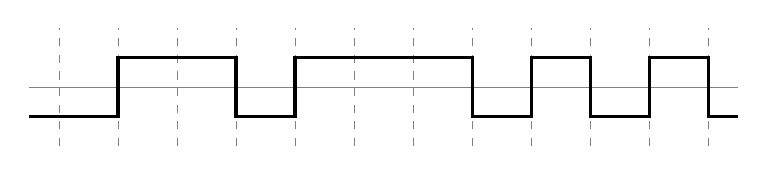
\begin{tikzpicture}[scale=0.75,transform shape]
            \draw[gray,very thin] (-0.5,6) -- (11.5,6);
            \foreach \x in {0,1,2,...,11}
            {
                \draw[gray,dashed,very thin] (\x,5) -- (\x,7);
            }
            \draw[black,very thick] (-0.5,5.5)--(1,5.5)--(1,6.5)--(3,6.5)--(3,5.5)--(4,5.5)--(4,6.5)--(7,6.5)--(7,5.5)--(8,5.5)--(8,6.5)--(9,6.5)--(9,5.5)--(10,5.5)--(10,6.5)--(11,6.5)--(11,5.5)--(11.5,5.5);
          \end{tikzpicture}
      \end{figure}
    \pause
    \item \only<7>{\sout}{$\text{PSD} = \pause \mathcal{F}\left[ R_u(\tau) \right]$} \only<7>{\alert{Neither SSS nor WSS}}
    \pause
  \end{itemize}
  \normalsize
\end{frame}

%% Frame %%
\begin{frame}{Cyclostationary Random Process}
  \footnotesize
  \pause
  \begin{definition}[Cyclostationary RP]
    A random process $X(t)$ is cyclostationary with respect to time interval $T$ if \pause it is statistically indistinguishable from $X(t-kT)$ for any integer $k$.
  \end{definition}
  \pause
  \begin{definition}[Wide Sense Cyclostationary RP]
    \pause
    A random process $X(t)$ is wide sense cyclostationary with respect to time interval $T$ if \pause the mean and autocorrelation functions satisfy
    \pause
    \begin{eqnarray*}
      m_X(t) & = & m_X(t-T) \ \ \ \ \text{for all } t,\\
      \pause
      R_X(t_1,t_2) & = & R_X(t_1-T,t_2-T) \ \ \ \ \text{for all } t_1,t_2.
    \end{eqnarray*}
  \end{definition}
  \normalsize
\end{frame}

%% Frame %%
\begin{frame}{Power Spectral Density of a Cyclostationary Process}
  \footnotesize
  To obtain the PSD of a cyclostationary process with period $T$
  \pause
  \begin{itemize}
    \item Calculate autocorrelation of cyclostationary process $R_X(t,t-\tau)$
    \pause
    \item Average autocorrelation between $0$ and $T$, $R_X(\tau) = \frac{1}{T} \int_0^T R_X(t,t-\tau) \ dt$
    \pause
    \item Calculate Fourier transform of averaged autocorrelation $R_X(\tau)$
  \end{itemize}
  \normalsize
\end{frame}

%% Frame %%
\begin{frame}{Power Spectral Density of a Realization}
  \footnotesize
  Time windowed realizations have finite energy
    \begin{eqnarray*}
      x_{T_o}(t) & = & x(t)I_{[-\frac{T_o}{2},\frac{T_o}{2}]}(t) \\
      \pause
      S_{T_o}(f) & = & \mathcal{F}(x_{T_o}(t)) \\
      \pause
      \hat{S}_x(f) & = & \frac{\lvert S_{T_o}(f) \rvert^2}{T_o} \ \ \ \ \text{ (PSD Estimate)}
    \end{eqnarray*}
  \pause
  \begin{block}{PSD of a realization}
    \begin{equation*}
    \bar{S}_x(f) = \lim_{T_o \rightarrow \infty} \frac{\lvert S_{T_o}(f) \rvert^2}{T_o}
    \end{equation*}
    \pause
    \begin{equation*}
\frac{\lvert S_{T_o}(f) \rvert^2}{T_o}  \xrightleftharpoons{}  \pause\frac{1}{T_o} \int_{-\frac{T_o}{2}}^{\frac{T_o}{2}} x_{T_o}(u)x_{T_o}^*(u-\tau) \ du \pause =\hat{R}_x(\tau)  
    \end{equation*}
  \end{block}
  \normalsize
\end{frame}

%% Frame %%
\begin{frame}{Power Spectral Density of a Cyclostationary Process}
  \footnotesize
  $X(t)X^*(t-\tau) \sim X(t+T)X^*(t+T-\tau)$ for cyclostationary $X(t)$
  \begin{eqnarray*}
    \hat{R}_x(\tau) & = & \frac{1}{T_o} \int_{-\frac{T_o}{2}}^{\frac{T_o}{2}} x(t)x^*(t-\tau) \ dt \\
    \pause
                    & = & \frac{1}{KT} \int_{-\frac{KT}{2}}^{\frac{KT}{2}} x(t)x^*(t-\tau) \ dt \ \ \ \ \ \ \ \   \text{for } T_o = KT\\
    \pause
                    & = & \frac{1}{T} \int_{0}^{T} \frac{1}{K} \sum_{k=-\frac{K}{2}}^{\frac{K}{2}}x(t+kT)x^*(t+kT-\tau) \ dt  \\
    \pause
                    & \underset{K \rightarrow \infty}{\longrightarrow} & \frac{1}{T} \int_{0}^{T} E\left[X(t)X^*(t-\tau)\right] \ dt  \\
    \pause
                    & = & \frac{1}{T} \int_{0}^{T} R_X(t,t-\tau) \ dt  \pause = R_X(\tau)
  \end{eqnarray*}
  \pause
  PSD of a cyclostationary process = $\mathcal{F}[R_X(\tau)]$ 
  \normalsize
\end{frame}

%% Frame %%
\begin{frame}{PSD of a Linearly Modulated Signal}
  \footnotesize
  \begin{itemize}
    \item Consider
      \begin{equation*}
        u(t) = \sum_{n=-\infty}^{\infty} b_n p(t-nT)
      \end{equation*}
    \pause
    \item $u(t)$ is cyclostationary wrt to $T$ if $\{b_n\}$ is stationary
    \pause
    \item $u(t)$ is wide sense cyclostationary wrt to $T$ if $\{b_n\}$ is WSS
    \pause
    \item Suppose $R_b[k] = E[b_{n} b_{n-k}^*]$
    \pause
    \item Let $S_b(z) = \sum_{k=-\infty}^{\infty} R_b[k]z^{-k}$
    \pause
    \item The PSD of $u(t)$ is given by
      \begin{equation*}
        S_u(f) = S_b\left(e^{\ j2\pi fT}\right)\frac{\lvert P(f)\rvert^2}{T}
      \end{equation*}
  \end{itemize}
  \normalsize
\end{frame}

%% Frame %%
\begin{frame}{PSD of a Linearly Modulated Signal}
  \footnotesize
  \begin{eqnarray*}
    \pause
    \lefteqn{R_u(\tau)}\\
        \pause
        & = & \frac{1}{T} \int_0^T R_u(t+\tau,t) \ dt \\
        \pause
        & = & \frac{1}{T}\int_0^T \sum_{n=-\infty}^{\infty} \sum_{m=-\infty}^{\infty} E\left[b_nb_m^*p(t-nT+\tau)p^*(t-mT) \right] \ dt\\
        %& = & \frac{1}{T}\sum_{k=-\infty}^{\infty} \sum_{m=-\infty}^{\infty} \int_0^T E\left[b_mb_n^*p(t-mT-kT+\tau)p^*(t-mT) \right] \ dt\\
        \pause
        & = & \frac{1}{T}\sum_{k=-\infty}^{\infty} \sum_{m=-\infty}^{\infty} \int_{-mT}^{-(m-1)T} E\left[b_{m+k}b_m^*p(\lambda-kT+\tau)p^*(\lambda) \right] \ d\lambda\\
        \pause
        & = & \frac{1}{T}\sum_{k=-\infty}^{\infty} \int_{-\infty}^{\infty} E\left[b_{m+k}b_m^*p(\lambda-kT+\tau)p^*(\lambda) \right] \ d\lambda\\
        \pause
        & = & \frac{1}{T}\sum_{k=-\infty}^{\infty} R_b[k]\int_{-\infty}^{\infty} p(\lambda-kT+\tau)p^*(\lambda)  \ d\lambda
  \end{eqnarray*}
  \normalsize
\end{frame}

%% Frame %%
\begin{frame}{PSD of a Linearly Modulated Signal}
  \footnotesize
  \begin{equation*}
    R_u(\tau) = \frac{1}{T}\sum_{k=-\infty}^{\infty} R_b[k]\int_{-\infty}^{\infty} p(\lambda-kT+\tau)p^*(\lambda)  \ d\lambda
  \end{equation*}
  \pause
  \begin{eqnarray*}
    \int_{-\infty}^{\infty} p(\lambda+\tau)p^*(\lambda)  \ d\lambda & \xrightleftharpoons{} & \pause \lvert P(f) \rvert^2 \\
    \pause
    \int_{-\infty}^{\infty} p(\lambda-kT+\tau)p^*(\lambda)  \ d\lambda & \xrightleftharpoons{} & \pause \lvert P(f) \rvert^2 e^{\ -j2\pi fkT} 
  \end{eqnarray*}
  \pause
  \begin{eqnarray*}
    S_u(f) = \pause \mathcal{F}\left[ R_u(\tau) \right] & = & \pause \frac{\lvert P(f)\rvert^2}{T}\sum_{k=-\infty}^{\infty} R_b[k] e^{\ -j2\pi fkT} \\
          & = & \pause S_b\left(e^{\ j2\pi fT}\right)\frac{\lvert P(f)\rvert^2}{T}
  \end{eqnarray*}
  where $S_b(z) = \sum_{k=-\infty}^{\infty} R_b[k]z^{-k}$.
  \normalsize
\end{frame}

\section{Power Spectral Density of Line Codes}

%% Frame %%
\begin{frame}{Line Codes}
  \footnotesize
  \begin{figure}
    \centering
      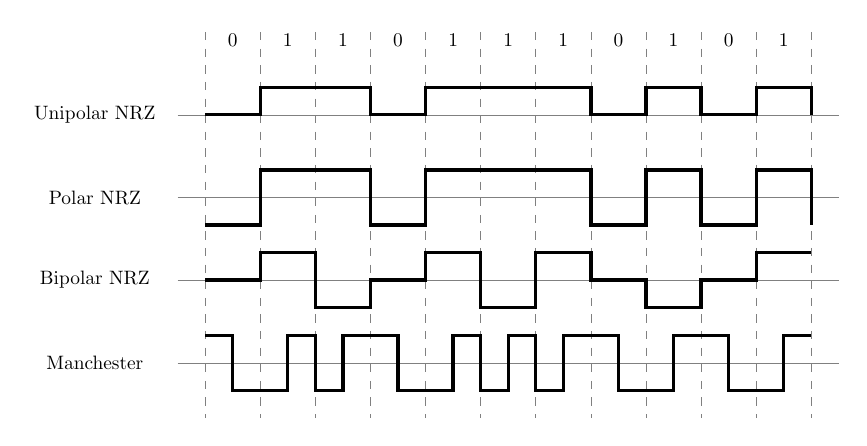
\begin{tikzpicture}[scale=0.7,transform shape]
        \node at (0.5,8.85) {0};
        \node at (1.5,8.85) {1};
        \node at (2.5,8.85) {1};
        \node at (3.5,8.85) {0};
        \node at (4.5,8.85) {1};
        \node at (5.5,8.85) {1};
        \node at (6.5,8.85) {1};
        \node at (7.5,8.85) {0};
        \node at (8.5,8.85) {1};
        \node at (9.5,8.85) {0};
        \node at (10.5,8.85) {1};
        \foreach \y in {3,4.5,6,7.5}
        {
            \draw[gray,very thin] (-0.5,\y) -- (11.5,\y);
        }
        \foreach \x in {0,1,2,...,11}
        {
            \draw[gray,dashed,very thin] (\x,9.) -- (\x,2);
        }
        \node at (-2,7.5) {Unipolar NRZ};
        \draw[black,very thick] (0,7.5)--(1,7.5)--(1,8)--(3,8)--(3,7.5)--(4,7.5)--(4,8)--(7,8)--(7,7.5)--(8,7.5)--(8,8)--(9,8)--(9,7.5)--(10,7.5)--(10,8)--(11,8)--(11,7.5);
        \pause
        \node at (-2,6) {Polar NRZ};
        \draw[black,very thick] (0,5.5)--(1,5.5)--(1,6.5)--(3,6.5)--(3,5.5)--(4,5.5)--(4,6.5)--(7,6.5)--(7,5.5)--(8,5.5)--(8,6.5)--(9,6.5)--(9,5.5)--(10,5.5)--(10,6.5)--(11,6.5)--(11,5.5);
        \pause
        \node at (-2,4.5) {Bipolar NRZ};
        \draw[black,very thick] (0,4.5)--(1,4.5)--(1,5)--(2,5)--(2,4)--(3,4)--(3,4.5)--(4,4.5)--(4,5)--(5,5)--(5,4)--(6,4)--(6,5)--(7,5)--(7,4.5)--(8,4.5)--(8,4)--(9,4)--(9,4.5)--(10,4.5)--(10,5)--(11,5);
        \pause
        \node at (-2,3) {Manchester};
        \draw[black,very thick] (0,3.5)--(0.5,3.5)--(0.5,2.5)--(1.5,2.5)--(1.5,3.5)--(2,3.5)--(2,2.5)--(2.5,2.5)--(2.5,3.5)--(3.5,3.5)--(3.5,2.5)--(3.5,2.5)--(4.5,2.5)--(4.5,3.5)--(5,3.5)--(5,2.5)--(5.5,2.5)--(5.5,3.5)--(6,3.5)--(6,2.5)--(6.5,2.5)--(6.5,3.5)--(7,3.5)--(7.5,3.5)--(7.5,2.5)--(8.5,2.5)--(8.5,3.5)--(9.5,3.5)--(9.5,2.5)--(10.5,2.5)--(10.5,3.5)--(11,3.5);
      \end{tikzpicture}
  \end{figure}
  \pause
  \only<5>{Further reading: \textit{Digital Communications}, Simon Haykin, Chapter 6}
  \normalsize
\end{frame}

%% Frame %%
\begin{frame}{Unipolar NRZ}
  \footnotesize
  \begin{itemize}
    \item Symbols independent and equally likely to be $0$ or $A$
      \begin{equation*}
        P\left(b[n] = 0\right) = P\left(b[n]= A\right) = \frac{1}{2}
      \end{equation*}
    \pause
    \item Autocorrelation of $b[n]$ sequence 
      \begin{equation*}
        R_b[k] = \left\{ 
                    \begin{array}{rr}
                      \pause
                      \frac{A^2}{2} & k = 0 \\
                          & \\
                      \pause
                      \frac{A^2}{4} & k \neq 0 
                    \end{array}
                 \right.
      \end{equation*}
    \pause 
    \item $p(t) = I_{[0,T)}(t)\Rightarrow P(f) = \pause T\text{sinc}(fT)\pause e^{\ -j\pi fT}$
    \pause
    \item Power Spectral Density
      \begin{equation*}
        S_u(f) = \frac{\lvert P(f)\rvert^2}{T}\sum_{k=-\infty}^{\infty} R_b[k] e^{\ -j2\pi kfT}
      \end{equation*}
  \end{itemize}
  \normalsize
\end{frame}

%% Frame %%
\begin{frame}{Unipolar NRZ}
  \footnotesize
  \begin{eqnarray*}
    S_u(f) & = & \frac{A^2T}{4}\text{sinc}^2(fT) + \frac{A^2T}{4}\text{sinc}^2(fT) \sum_{k=-\infty}^{\infty}  e^{\ -j2\pi kfT} \\
    \pause
           & = & \frac{A^2T}{4}\text{sinc}^2(fT) + \frac{A^2}{4}\text{sinc}^2(fT) \sum_{n=-\infty}^{\infty}  \delta\left(f - \frac{n}{T}\right) \\
    \pause
           & = & \frac{A^2T}{4}\text{sinc}^2(fT) + \frac{A^2}{4} \delta(f) 
  \end{eqnarray*}
  \normalsize
\end{frame}

%% Frame %%
\begin{frame}{Normalized PSD plot}
  \footnotesize
  \begin{figure}
    \centering
      \begin{tikzpicture}[scale=1.0,transform shape]
        \begin{axis}[xlabel=$fT$, ylabel=$\frac{S_u(f)}{A^2T}$,xmax=2,xmin=0.01,ymax=1,ymin=-0.05,grid=major,x post scale = 1.3, xtick={0.5,1,1.5,2}, ytick={0,0.5,1}]
          \addplot[color=blue,very thick,domain=0.01:2,samples=1000] gnuplot{0.25*(sin(pi*x)/(pi*x))*(sin(pi*x)/(pi*x))};
          \draw[blue,->,very thick] (axis cs:0.01,0) -- (axis cs:0.01,0.35);
          \addlegendentry{Unipolar NRZ}
        \end{axis}
      \end{tikzpicture}
  \end{figure}
  \normalsize
\end{frame}

%% Frame %%
\begin{frame}{Polar NRZ}
  \footnotesize
  \begin{itemize}
    \item Symbols independent and equally likely to be $-A$ or $A$
      \begin{equation*}
        P\left(b[n] = -A\right) = P\left(b[n]= A\right) = \frac{1}{2}
      \end{equation*}
    \pause
    \item Autocorrelation of $b[n]$ sequence 
      \begin{equation*}
        R_b[k] = \left\{ 
                    \begin{array}{rr}
                      \pause
                       A^2 & k = 0 \\
                          & \\
                      \pause
                       0 & k \neq 0 
                    \end{array}
                 \right.
      \end{equation*}
    \pause 
    \item $P(f) = T\text{sinc}(fT) e^{\ -j\pi fT}$
    \pause
    \item Power Spectral Density
      \begin{equation*}
        S_u(f) = \pause A^2T\text{sinc}^2(fT) 
      \end{equation*}
  \end{itemize}
  \normalsize
\end{frame}

%% Frame %%
\begin{frame}{Normalized PSD plots}
  \footnotesize
  \begin{figure}
    \centering
      \begin{tikzpicture}[scale=1.0,transform shape]
        \begin{axis}[xlabel=$fT$, ylabel=$\frac{S_u(f)}{A^2T}$,xmax=2,xmin=0.01,ymax=1,ymin=-0.05,grid=major,x post scale = 1.3, xtick={0.5,1,1.5,2}, ytick={0,0.5,1}]
          \addplot[color=blue,very thick,domain=0.01:2,samples=1000] gnuplot{0.25*(sin(pi*x)/(pi*x))*(sin(pi*x)/(pi*x))};
          \draw[blue,->,very thick] (axis cs:0.01,0) -- (axis cs:0.01,0.35);
          \addlegendentry{Unipolar NRZ}
          \addplot[color=red,very thick,domain=0.01:2,samples=1000] gnuplot{(sin(pi*x)/(pi*x))*(sin(pi*x)/(pi*x))};
          \addlegendentry{Polar NRZ}
        \end{axis}
      \end{tikzpicture}
  \end{figure}
  \normalsize
\end{frame}

%% Frame %%
\begin{frame}{Manchester}
  \footnotesize
  \begin{itemize}
    \item Symbols independent and equally likely to be $-A$ or $A$
      \begin{equation*}
        P\left(b[n] = -A\right) = P\left(b[n]= A\right) = \frac{1}{2}
      \end{equation*}
    \pause
    \item Autocorrelation of $b[n]$ sequence 
      \begin{equation*}
        R_b[k] = \left\{ 
                    \begin{array}{rr}
                      \pause
                       A^2 & k = 0 \\
                          & \\
                      \pause
                       0 & k \neq 0 
                    \end{array}
                 \right.
      \end{equation*}
    \pause 
    \item $P(f) = \pause jT\text{sinc}\left(\frac{fT}{2}\right) \sin \left(\frac{\pi fT}{2}\right)e^{-j\pi fT}$
    \pause
    \item Power Spectral Density
      \begin{equation*}
        S_u(f) = \pause A^2T\text{sinc}^2\left(\frac{fT}{2}\right) \sin^2 \left(\frac{\pi fT}{2}\right)
      \end{equation*}
  \end{itemize}
  \normalsize
\end{frame}

%% Frame %%
\begin{frame}{Normalized PSD plots}
  \footnotesize
  \begin{figure}
    \centering
      \begin{tikzpicture}[scale=1.0,transform shape]
        \begin{axis}[xlabel=$fT$, ylabel=$\frac{S_u(f)}{A^2T}$,xmax=2,xmin=0.01,ymax=1,ymin=-0.05,grid=major,x post scale = 1.3, xtick={0.5,1,1.5,2}, ytick={0,0.5,1}]
          \addplot[color=blue,very thick,domain=0.01:2,samples=1000] gnuplot{0.25*(sin(pi*x)/(pi*x))*(sin(pi*x)/(pi*x))};
          \draw[blue,->,very thick] (axis cs:0.01,0) -- (axis cs:0.01,0.35);
          \addlegendentry{Unipolar NRZ}
          \addplot[color=red,very thick,domain=0.01:2,samples=1000] gnuplot{(sin(pi*x)/(pi*x))*(sin(pi*x)/(pi*x))};
          \addlegendentry{Polar NRZ}
          \addplot[color=black,very thick,domain=0.01:2,samples=1000] gnuplot{(sin(pi*x/2)/(pi*x/2))*(sin(pi*x/2)/(pi*x/2))*sin(pi*x/2)*sin(pi*x/2)};
          \addlegendentry{Manchester}
        \end{axis}
      \end{tikzpicture}
  \end{figure}
  \normalsize
\end{frame}

%% Frame %%
\begin{frame}{Bipolar NRZ}
  \footnotesize
  \begin{itemize}
    \item Successive 1's have alternating polarity
      \begin{eqnarray*}
          0 & \rightarrow &\text{Zero amplitude} \\
          1 & \rightarrow &  +A \text{ or } -A
      \end{eqnarray*}
    \pause
    \item Probability mass function of $b[n]$
      \begin{eqnarray*}
        P\left(b[n] = 0\right) & = & \pause \frac{1}{2}\\
        P\left(b[n] = -A\right) & = & \pause \frac{1}{4}\\
        P\left(b[n] = A\right) & = & \pause \frac{1}{4}
      \end{eqnarray*}
    \pause
    \item Symbols are identically distributed but they are not independent
  \end{itemize}
  \normalsize
\end{frame}

%% Frame %%
\begin{frame}{Bipolar NRZ}
  \footnotesize
  \begin{itemize}
    \item Autocorrelation of $b[n]$ sequence 
      \begin{equation*}
        R_b[k] = \left\{ 
                    \begin{array}{rl}
                       \pause
                       A^2/2 & \ \ \ \ \ \ \ k = 0 \\
                       \pause
                       -A^2/4 & \ \ \ \ \ \ \ k = \pm 1 \\
                       \pause
                       0 & \ \ \ \ \ \ \ \text{otherwise}
                    \end{array}
                 \right.
      \end{equation*}
    \pause
    \item Power Spectral Density
      \begin{eqnarray*}
        S_u(f) & = & T\text{sinc}^2(fT)\left[ \frac{A^2}{2} - \frac{A^2}{4}\left(e^{\ j2\pi fT} + e^{\ -j2\pi fT}\right)\right]  \\
        \pause
               & = &  \frac{A^2T}{2}\text{sinc}^2(fT)\left[1-\cos(2\pi fT) \right]\\
        \pause
               & = & A^2T\text{sinc}^2(fT)\sin^2(\pi fT)
      \end{eqnarray*}
  \end{itemize}
  \normalsize
\end{frame}

%% Frame %%
\begin{frame}{Normalized PSD plots}
  \footnotesize
  \begin{figure}
    \centering
      \begin{tikzpicture}[scale=1.0,transform shape]
        \begin{axis}[xlabel=$fT$, ylabel=$\frac{S_u(f)}{A^2T}$,xmax=2,xmin=0.01,ymax=1,ymin=-0.05,grid=major,x post scale = 1.3, xtick={0.5,1,1.5,2}, ytick={0,0.5,1}]
          \addplot[color=blue,very thick,domain=0.01:2,samples=1000] gnuplot{0.25*(sin(pi*x)/(pi*x))*(sin(pi*x)/(pi*x))};
          \draw[blue,->,very thick] (axis cs:0.01,0) -- (axis cs:0.01,0.35);
          \addlegendentry{Unipolar NRZ};
          \addplot[color=red,very thick,domain=0.01:2,samples=1000] gnuplot{(sin(pi*x)/(pi*x))*(sin(pi*x)/(pi*x))};
          \addlegendentry{Polar NRZ};
          \addplot[color=black,very thick,domain=0.01:2,samples=1000] gnuplot{(sin(pi*x/2)/(pi*x/2))*(sin(pi*x/2)/(pi*x/2))*sin(pi*x/2)*sin(pi*x/2)};
          \addlegendentry{Manchester};
          \addplot[color=orange,very thick,domain=0.01:2,samples=1000] gnuplot{(sin(pi*x)/(pi*x))*(sin(pi*x)/(pi*x))*sin(pi*x)*sin(pi*x)};
          \addlegendentry{Bipolar NRZ};
        \end{axis}
      \end{tikzpicture}
  \end{figure}
  \normalsize
\end{frame}

%% Frame %%
\begin{frame}{}
\vfill
\begin{center}
Thanks for your attention
\end{center}
\vfill
\end{frame}

\end{document}
